\chapter{Multi-robot Relative Pose Initialization}
\label{chap:four}

In this chapter, we address the problem of global consistency in the estimated values of the decision variables in least squares optimization \textit{across multiple robots.} The problem roughly boils down to initialization of the robot's relative pose in case of an encounter. Providing a good prior over the starting point of all robots that are consistent with respect to an external global frame partially solves the problem. However, it is a daunting task and also the presence of inter-robot constraints will further refine the estimates of the starting point of the robots. These inter-robot constraints are provided by introducing the ``global nail", that transforms the trajectory of any individual robot to global frame, as an estimation variable. By doing this, we demonstrate the alignment of map reconstructed by every robot based on the optimized trajectory. The next section briefly discusses the related work. Following that, we describe our proposed methodology. 

\section{Related Work}
Although the field of multi-robot SLAM has been explored significantly \cite{multi1, multi2, multi3, thrunmulti}, there is only a small body of work available on graph based multi-robot mapping. The problem of initialization of relative poses are addressed differently within various frameworks with qualifying assumptions. Early work in multi-robot mapping like \cite{multi3} assume known starting pose of all the robots with certainty in advance. A slight development in \cite{howardmulti} incorporates the initialization problem within the mapping framework but assumes that the very first encounter is perfect and hence neglects the subsequent encounters. It further developed into acknowledging the importance of initialization in \cite{thrunmulti} and consequently addressing it using the sparse extended information filter. In the context of smoothing and mapping (SAM), the most related work include cooperative SAM (C-SAM) \cite{csam}, tectonic SAM (T-SAM) \cite{tectonicsam} and multiple pose graph SLAM \cite{multipleisam}. Tectonic SAM is based on the similar principle that has the global nail to represent relative pose across different submaps of the region. It is batch algorithm for single robot. C-SAM is a batch algorithm for cooperative mapping and is tested only on simulation using two robots. Multiple pose graph SLAM is the one closest to our approach but does not explicitly consider the loop closures and landmarks while merging the pose graphs. 
 
\section{Relative Factor Graph Initialization} 
It is not necessary that all the robots in a multi-robot scenario start at the same location as assumed by several previous works. Figure \ref{fig:pose_graphs} shows the factor graph of three different robots. The factor graphs in this particular example can be considered to encode spatial information of the robot's trajectory and can be seen that they start at different positions and overlap. An arbitrary value as a prior factor over the starting pose works completely fine until a first direct encounter between the robots or indirect encounter by multiple robots visiting the same portion of the environment. The factor graph representation of a bunch of direct and indirect encounters is given in Figure \ref{fig:pose_graphs_encounter}. It is during this event that there is a conflict between the estimates of the state variables across different graphs and the measured local value of the encounter. This problem is resolved by introducing the ``global nail" for every individual robot's factor graph that converts the pose variable estimate locally consistent with the prior to the common global reference frame. Figure \ref{fig:pose_graphs_nails} introduces the global nails that constrain multiple robot trajectories using the relative transform from every robot frame to the common global frame. That said, the introduction of global nails might seem to remove the need for prior over the initial variables. Removing the prior does not affect the local measurements between variables but it will provide a gauge freedom for all the individual robot’s factor graphs. This is extremely problematic because the good linearization point can be far away from the variable estimates and any iterative optimization has the unintended consequence of getting stuck in the local minima. Thus the prior over the initial variables and the global nails are both essential to estimate the states of all the robots departing from various and uncertain starting locations. 
\begin{figure}
\centering
\includegraphics[width=\textwidth]{Chapters/figures4/pose_graph}
\caption{Factor graphs of three different robots. For this example, it can be considered that they also represent the spatial information of the trajectory.}
\label{fig:pose_graphs}
\end{figure}
\begin{figure}
\centering
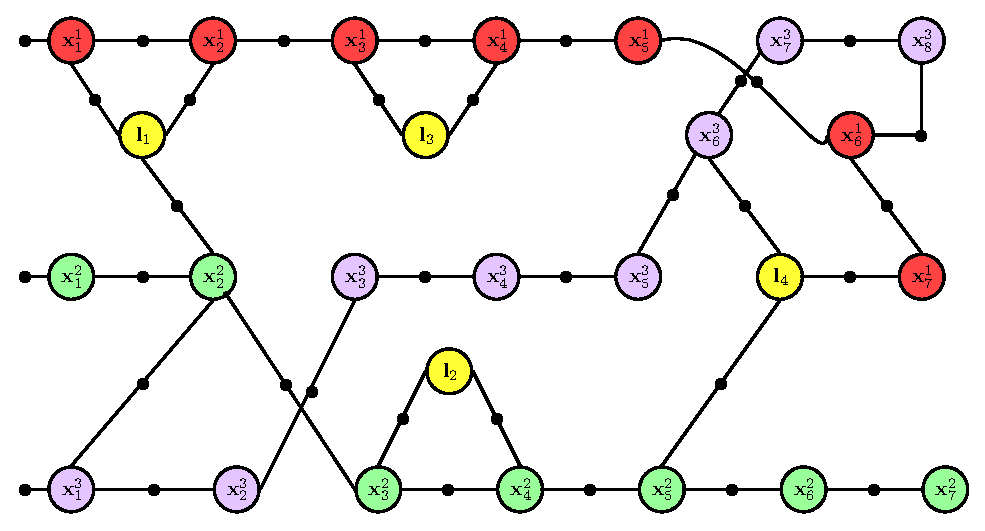
\includegraphics[width=\textwidth]{Chapters/figures4/pose_graph_encounters}
\caption{The set of direct and indirect encounters between robots in their overlapping trajectories are expressed. An indirect encounter is landmark connecting two different factor graphs and direct encounter is shown by a factor directly connecting two different factor graphs.}
\label{fig:pose_graphs_encounter}
\end{figure}
\begin{figure}
\centering
\includegraphics[width=\textwidth]{Chapters/figures4/pose_graph_with_nail}
\caption{The same encounters as in the previous figure but using the relative factor graph formulation. A global nail $T_r^G$ is introduced for each trajectory that specify the offset with respect to the global frame. All the encounters are connected with the global nail to account for multiple, uncertain encounters converging towards optimal solution over time.}
\label{fig:pose_graphs_nails}
\end{figure}
 
\paragraph{}
Using the global nail transforms the respective poses of each pose graph into a common global reference frame where the comparison becomes possible. This is illustrated using an example encounter in Figure \ref{fig:err_func}. The transform $T_G^1$ and $T_G^2$ are optimized such that the following equation representing the error on $l_1$ is as low as possible:
\begin{equation}
T_1^GT_{x_1^1}^1l_1^{x_1^1} - T_{2}^GT_{x_{2}^{2}}^{2}l_1^{x_{2}^{2}}
\label{eq:err_func_example}
\end{equation}
\begin{figure}[H]
\centering
\includegraphics{Chapters/figures4/err_func}
\caption{Labelling the parts of a single encounter to understand the formulation of global nail factor.}
\label{fig:err_func}
\end{figure}
In the above Equation \ref{eq:err_func_example} the terms $l_1^{x_1^1}$ and $l_1^{x_{2}^{2}}$ are obtained from the sensor measurements like fiducial detection as explained in the next chapter. The terms $T_{x_1^1}^1$ and $T_{x_{2}^{2}}^{2}$ are the direct reflection of the value of prior over the initial variable of each factor graph and $T_1^G$ and $T_{2}^G$ are the variables to be estimated. The new type of factor that relates the encounter measurement along with the global nail is mathematically formulated as follows:
\begin{equation}
\sum_{n=1}^N \bigg\lvert\bigg\lvert T_r^GT_{x_i^r}^rl_n^{x_i^r} - T_{r^\prime}^GT_{x_{i^\prime}^{r^\prime}}^{r^\prime}l_n^{x_{i^\prime}^{r^\prime}}\bigg\rvert\bigg\rvert_{\Gamma_n}^2
\label{eq:err_func}
\end{equation}
where $r$ and $r^\prime$, $i$ and $i^\prime$ are the indices of robot and robot poses. $\Lambda_n$ denotes the corresponding direct or indirect encounter covariance. The above error function to be minimized is added to the least squares formulation in Equation \ref{eq:multilinlsopt} incrementally for every encounter. 
\paragraph{}
Now it should be noted that the overall system encompassing all the factor graphs faces gauge freedom. This is restricted by adding a prior over the first global nail. All the other global nails are added as they are needed. Generally, the covariance of the prior is made large because it is very likely to conflict when there is an encounter. The alignment of the maps and the improvement in the estimation quality is discussed and displayed in Chapter \ref{chap:six}.
